\chapter{Modulador 16-QAM}
\label{section:qam}


En este Capítulo se muestra el bloque encargado de la modulación 16-QAM. Este bloque se compone de tres procesos: mapeado 16-QAM, aplicación de Zero Padding y filtrado \textit{Root Raised Cosine}. En la Figura \ref{fig:qam_fir} se puede visualizar la estructura de los bloques IP que se han incluido en este segundo proyecto de Vivado. 

\vspace{2mm}

\begin{figure}[h]
	\centering
	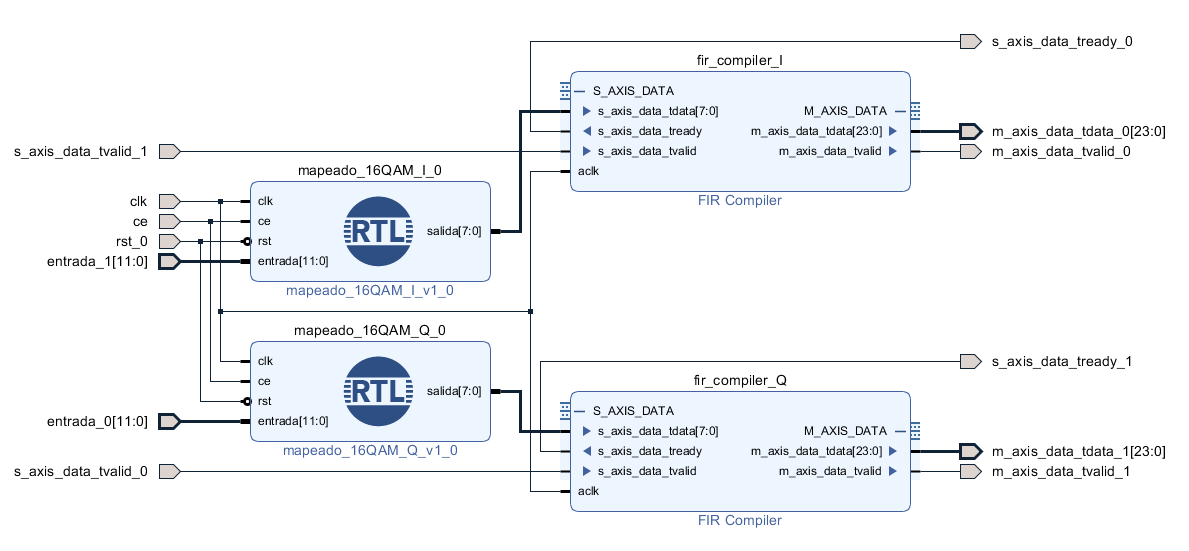
\includegraphics[width=1\textwidth]{img/diseno/qam_fir.PNG}
	\caption{Diseño de los bloques mapeado 16-QAM + ZP y filtrado RRC}
	\label{fig:qam_fir}
\end{figure}
    
\vspace{1mm}

\section{Mapeado 16-QAM}

\subsection{Configuración del mapeado 16-QAM}

Para implementar una modulación 16-QAM (Modulación de Amplitud en Cuadratura) lo primero que se debe realizar es el bloque de mapeado, con el fin de asignar patrones de amplitud y fase a cada símbolo y proporcionar una mayor eficiencia espectral. 

\pagebreak

Para ello, se recibe una señal de entrada de 12 bits, obtenida a partir de la lectura de los 200 valores almacenados en la memoria FIFO. Se debe crear un proceso en el testbench que se ejecute en cada ciclo del reloj global, configurado a 192MHz, que realice la lectura del fichero \textit{FIFO\_out.txt}. 

Como se había descrito en el Apartado \ref{section:fifo}, se escriben en dicho fichero los valores almacenados en la memoria FIFO para emplearlo como la entrada del bloque de mapeado 16-QAM y optimizar así los proyectos de Vivado.

\vspace{5mm}

\begin{lstlisting}[language=VHDL, style=mystyle, caption={Proceso de lectura del fichero FIFO\_out.txt}]
	process(clk) --192MHz
    variable line_buffer : line;
    variable nuevo_valor : STD_LOGIC_VECTOR(11 DOWNTO 0);
    
    begin
        if rst_0 = '1' then
            eof <= false; --se reinicia fin de archivo
            cont_in <= 0;
        elsif rising_edge(clk) then
            cont_in <= cont_in + 1;
            if cont_in = 96 then --cada 500 ns se lee entrada
                cont_in <= 0;
                if not eof then
                    if endfile(file_handle) then 
                        eof <= true; 
                    else
                        readline(file_handle, line_buffer);
                        read(line_buffer, nuevo_valor);
                        entrada <= nuevo_valor;
                    end if;
                end if;
            end if;                      
        end if;
end process;  
\end{lstlisting}

\vspace{3mm}

Es importante tener en cuenta que la lectura se produce a una frecuencia de 2MHz, por lo que se debe añadir un contador de 96 ciclos en el proceso, además de comprobar si el fichero ha llegado al final. Según las especificaciones de este proyecto, la salida del mapeado debe funcionar a una frecuencia de 6MHz, es decir, el triple de la anterior porque por cada valor a la entrada de 12 bits se obtendrán 3 símbolos 16-QAM. En otros términos, se tratarán los bits de entrada de 4 en 4 para mapear cada símbolo 16-QAM. 

El mapeado de cada símbolo 16-QAM supone la generación a la salida de dos caminos independientes: uno para la componente en Fase (I) y otro para la de Cuadratura (Q). Cada símbolo es de 3 bits con signo y puede tomar los valores (-3,-1,+1,+3) como se puede visualizar en la Figura \ref{fig:qam}, procedente del ejemplo simulado en Matlab.

\pagebreak

\begin{figure}[h]
	\centering
	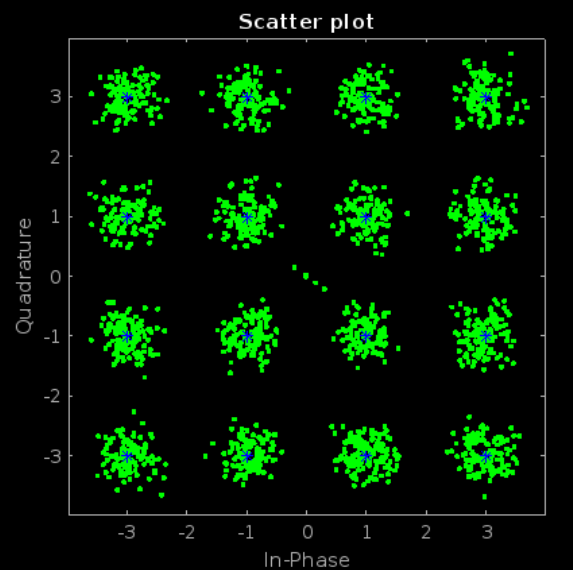
\includegraphics[width=0.45\textwidth]{img/matlab/qam.PNG}
	\caption{Constelación 16-QAM}
	\label{fig:qam}
\end{figure}

\vspace{3mm}
   
En este caso, se han decidido ajustar las tablas Q e I para establecer una codificación Gray. Esta se trata de una técnica específica que garantiza que solo un bit cambie entre dos valores consecutivos. Además, consigue minimizar la posibilidad de errores producidos por cambios de múltiples bits en la transmisión. A continuación, se puede visualizar la definición de cada una de las tablas:

\vspace{3mm}

\begin{lstlisting}[language=VHDL, style=mystyle, caption={Definición de la tabla de mapeado Q}]
type Array3Bit is array (0 to 15) of STD_LOGIC_VECTOR(2 downto 0);
constant tabla_mapeado_Q: Array3Bit :=
		("000", "001", "011", "010", 
		"110", "111", "101", "100",
		"000", "001", "011", "010", 
		"110", "111", "101", "100");
\end{lstlisting}

\vspace{5mm}

\begin{lstlisting}[language=VHDL, style=mystyle, caption={Definición de la tabla de mapeado I}]
type Array3Bit is array (0 to 15) of STD_LOGIC_VECTOR(2 downto 0);
constant tabla_mapeado_I: Array3Bit := 
	("000", "000", "001", "001", 
	"011", "011", "010", "010",
	"110", "110", "111", "111", 
	"101", "101", "100", "100");
\end{lstlisting}

\pagebreak

\section{Proceso de mapeado + Zero Padding}

\subsection{Configuración del proceso de mapeado + Zero Padding}

Además de implementar el mapeado 16-QAM, se añade en el bloque el zero-padding para optimizar el sistema de comunicación. Se insertan ceros a la señal original y se extiende su duración, aplicando en este caso una relación 1:32. Por lo tanto, por cada flanco en el que se transmita información, le seguirán 31 flancos en los que se transmitan bits con valor cero.

Por tanto, siguiendo las especificaciones anteriores, se decide combinar el mapeado 16-QAM con el zero-padding en un mismo bloque, para así obtener a la salida del mismo los símbolos 16-QAM con el Zero Padding ya aplicado. Así, se garantiza que la señal tenga una duración suficiente para conseguir una respuesta de frecuencia óptima, además de minimizar la interferencia entre símbolos. De forma adicional, se ajusta la salida a una longitud de 8 bits para dejarla preparada para la entrada del filtro pulse shaping del \textit{Root Raised Cosine} (RRC). 

\vspace{3mm}

\begin{lstlisting}[language=VHDL, style=mystyle, caption={Proceso de mapeado (Camino I) + Zero Padding}]
process(clk) 
	variable contador : integer := 0; -- 4*contador+3 downto 4*contador
	variable cont_32 : integer := 0; -- 6MHz
	variable captured_bits : std_logic_vector(3 downto 0) := "0000";
	variable aux_salida : std_logic_vector(2 downto 0):= "000";
begin
	if rising_edge(clk) then
		if rst = '1' then
			contador := 0; 
			cont_32 := 0; 
			salida <= (others => '0'); 
		else
			if cont_32 = 32 then -- se saca simbolo por la salida
				cont_32 := 0;
				captured_bits := entrada(4*contador+3 downto 4*contador);
				aux_salida := tabla_mapeado_I(to_integer(unsigned(captured_bits))); 
				--salida extendida a 8 bits
				salida(2 downto 0) <= aux_salida; 
				salida(7 downto 3) <= (others => aux_salida(2));
				contador := contador + 1; 
				if contador = 3 then 
					contador := 0; 
				end if;
			else --Zero Padding
				cont_32 := cont_32 + 1;
				salida <= (others => '0');
			end if;
		end if;
	end if;         
end process; 
\end{lstlisting}

\pagebreak

Como se puede visualizar, el proceso emplea dos contadores: uno para extraer en cada flanco los bits capturados de 4 en 4 e implementar el mapeado QAM para obtener los símbolos de 3 bits y otro para implementar la relación 1:32 respectiva al Zero Padding.

\subsection{Comprobación del proceso de mapeado + Zero Padding}

En las Figuras \ref{fig:proc2}, \ref{fig:proc3} y \ref{fig:proc1} se puede apreciar cómo se implementa el bloque de mapeado 16-QAM + zero-padding a través del proceso expuesto anteriormente.

\vspace{3mm}

\begin{figure}[h]
	\centering
	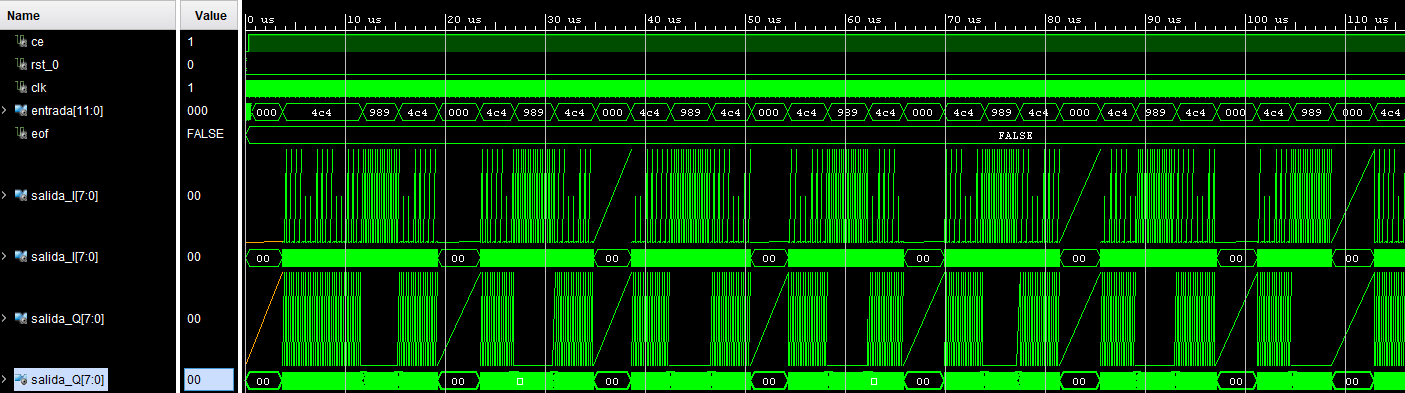
\includegraphics[width=1\textwidth]{img/simu/process_qam_2.PNG}
	\caption{Simulación completa del proceso de mapeado 16-QAM + ZP}
	\label{fig:proc2}
\end{figure}

\vspace{3mm}

\begin{figure}[h]
	\centering
	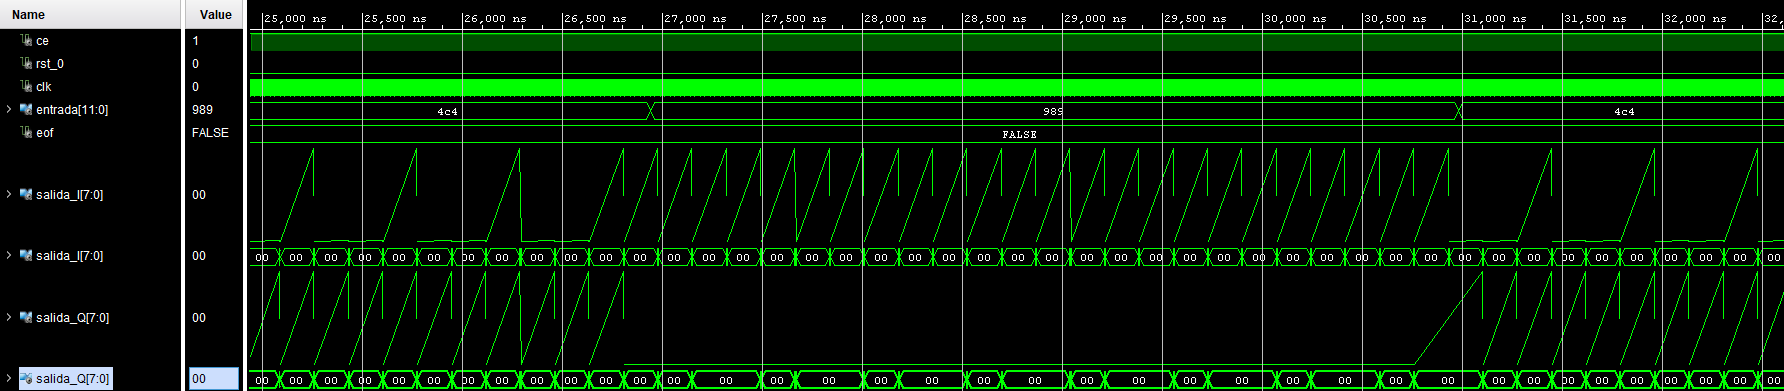
\includegraphics[width=1\textwidth]{img/simu/process_qam_3.PNG}
	\caption{Simulación del proceso de mapeado 16-QAM + ZP (II) (zoom medio)}
	\label{fig:proc3}
\end{figure}

\vspace{3mm}

\begin{figure}[h]
	\centering
	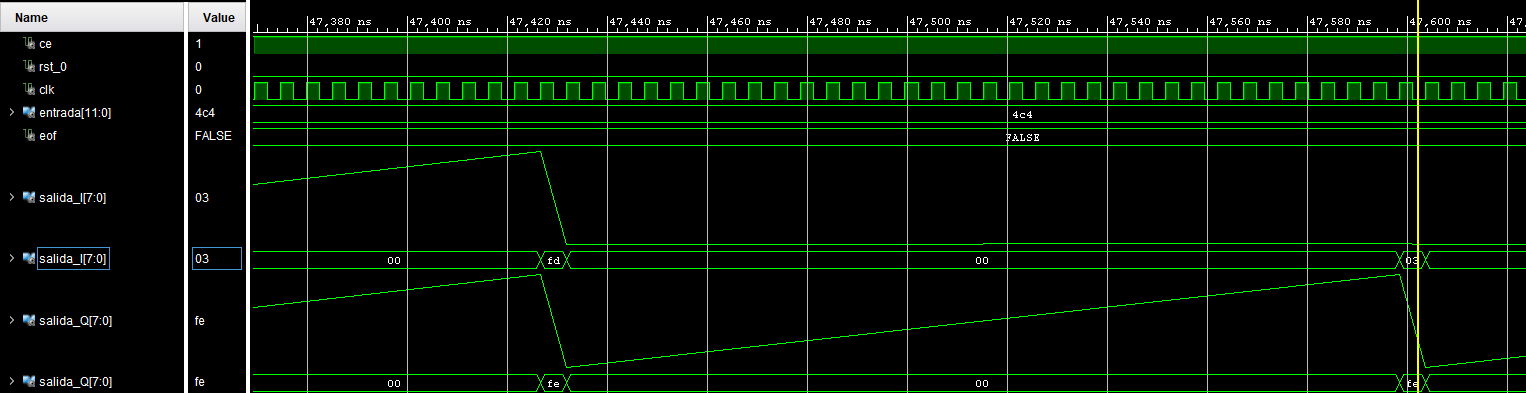
\includegraphics[width=1\textwidth]{img/simu/process_qam.PNG}
	\caption{Simulación del proceso de mapeado 16-QAM + ZP (III) (zoom alto)}
	\label{fig:proc1}
\end{figure}

\pagebreak

\vspace{3mm}

\section{Bloque de filtrado pulse shaping - RRC}

\subsection{Configuración del filtro RRC}

El filtro pulse shaping del \textit{Root Raised Cosine} (RRC) es un tipo de filtro denominado de coseno elevado. Se emplea en sistemas de comunicación digital para dar forma de onda a los pulsos que se transmiten. Minimiza la interferencia entre símbolos adyacentes y maximiza la eficiencia del espectro.

El primer paso a seguir para crear el filtro RRC es obtener los coeficientes del mismo. Para ello, se va a emplear Matlab, estableciendo de la siguiente forma las especificaciones del filtro a diseñar:

\vspace{5mm}

\begin{lstlisting}[language=matlab, style=mystyle, caption={Diseño del filtro RRC en Matlab}]
filtlen = 6;      % Longitud del filtro en numero de simbolos
rolloff = 0.25;   % Factor de rolloff para controlar el ancho del pulso
sps = 32;         % Muestras por simbolo (factor de oversampling)

rrcFilter = rcosdesign(rolloff,filtlen,sps);
fvtool(rrcFilter,'Analysis','Impulse')
\end{lstlisting}

\vspace{3mm}

Tras ejecutar el código, se obtendrán en total 193 coeficientes. Esto tiene como consecuencia que, para aplicar el filtro a la señal de entrada se irá ajustando un enventanado de longitud igual a 193 datos (dato actual + 192 datos siguientes) hasta finalizar la etapa. 

\vspace{3mm}

\begin{figure}[h]
	\centering
	\includegraphics[width=1\textwidth]{img/matlab/rrc.PNG}
	\caption{Respuesta al impulso del filtro RRC}
	\label{fig:fvtool}
\end{figure}
    
\vspace{3mm}

Mediante la herramienta gráfica \textit{fvtool} que proporciona Matlab se puede obtener la respuesta impulsiva del filtro RRC tal y como se muestra en la Figura \ref{fig:fvtool}.

\pagebreak

Para añadir el bloque del filtro en Vivado se requiere conocer el número de bits de los coeficientes, tanto de la parte entera como de la parte fraccionaria. Para ello, se emplea el comando de MatLab \textit{sfi(rrcFilter)} y se obtiene la salida de la Figura \ref{fig:fvtool2}

\vspace{3mm}

\begin{figure}[h]
	\centering
	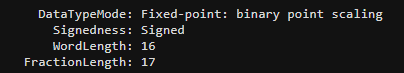
\includegraphics[width=0.6\textwidth]{img/matlab/coefs.PNG}
	\caption{Información sobre la matriz de coeficientes del filtro RRC}
	\label{fig:fvtool2}
\end{figure}
    
\vspace{3mm}

Como los coeficientes se encuentran dentro de un rango de valores entre 0 y 1, se establecen 16 bits para la logitud total y 17 bits, para la parte fraccionaria. Por otro lado, se configura el modo de truncamiento, una salida de filtrado de 24 bits y una entrada de 8 bits, que ya ha sido previamente ajustada en el bloque anterior, por lo que no se requieren procesos adicionales.

\vspace{3mm}

\begin{figure}[h]
	\centering
	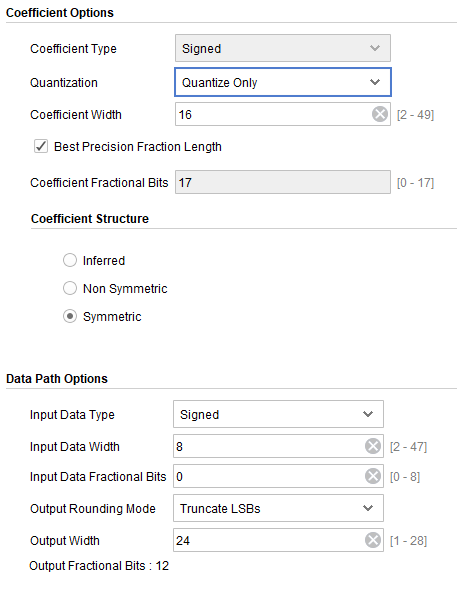
\includegraphics[width=0.65\textwidth]{img/diseno/fir.PNG}
	\caption{Configuración del filtro en Vivado}
	\label{fig:fvtool2}
\end{figure}
    
\pagebreak

Entrando en el código, para que el filtrado comience a operar es necesario primero resetear las entradas de validación de datos \textit{s\_axis\_data\_tvalid} de ambos filtros (camino I y Q) y después, activarlas cuando la señal de \textit{clock enable} se pone a 1. 

Por otro lado, como se había realizado con la salida de la memoria FIFO, para el bloque de filtrado también se van a almacenar los valores de salida en un fichero .txt. Para ello, se emplea el proceso definido anteriormente para la lectura de la FIFO y se añaden las líneas necesarias de escritura de los nuevos ficheros.

\vspace{5mm}

\begin{lstlisting}[language=vhdl, style=mystyle, caption={Proceso de escritura de los ficheros FIR\_output\_I.txt y FIR\_output\_Q.txt}]
process(clk) --192MHz
    --lectura datos FIFO
    variable line_buffer : line;
    variable nuevo_valor : STD_LOGIC_VECTOR(11 DOWNTO 0);
    
    --escritura datos FIR
    variable line_buffer_I, line_buffer_Q : line;
    variable nuevo_valor_I, nuevo_valor_Q : integer;
    
    begin
        if rst_0 = '1' then
            eof <= false; --se reinicia fin de archivo
            cont_in <= 0;
        elsif rising_edge(clk) then
            cont_in <= cont_in + 1;
            if cont_in = 96 then --cada 500 ns se lee entrada 
                cont_in <= 0;
                if not eof then
                    if endfile(file_handle) then 
                        eof <= true; 
                    else
                        readline(file_handle, line_buffer);
                        read(line_buffer, nuevo_valor);
                        entrada <= nuevo_valor;
                    end if;
                end if;
            end if; 
            if s_axis_data_tvalid_0 = '1' and s_axis_data_tvalid_1 = '1' and not eof then 
                --escritura de salida FIR I a 192MHz
                nuevo_valor_I:=to_integer(signed(m_axis_data_tdata_0));
                write(line_buffer_I, nuevo_valor_I); 
                writeline(file_handle_I, line_buffer_I); 
                --escritura de salida FIR Q a 192MHz
                nuevo_valor_Q:=to_integer(signed(m_axis_data_tdata_1));
                write(line_buffer_Q, nuevo_valor_Q); 
                writeline(file_handle_Q, line_buffer_Q);
            end if;                      
        end if;
end process; 
\end{lstlisting}

\pagebreak

\subsection{Comprobación del filtrado RRC}

En las Figuras \ref{fig:rrc1} y \ref{fig:rrc2} se visualiza la simulación completa del proyecto que incluye los bloques de mapeado 16-QAM + zero-padding y filtrado RRC. Se puede comprobar cómo el filtro da forma de onda a los pulsos que se transmiten y que provienen del proceso de mapeado previo.

\begin{figure}[h]
	\centering
	\includegraphics[width=1\textwidth]{img/simu/rrc.PNG}
	\caption{Simulación de los bloques de mapeado 16-QAM + ZP y filtrado RRC (I)}
	\label{fig:rrc1}
\end{figure}

\vspace{3mm}

\begin{figure}[h]
	\centering
	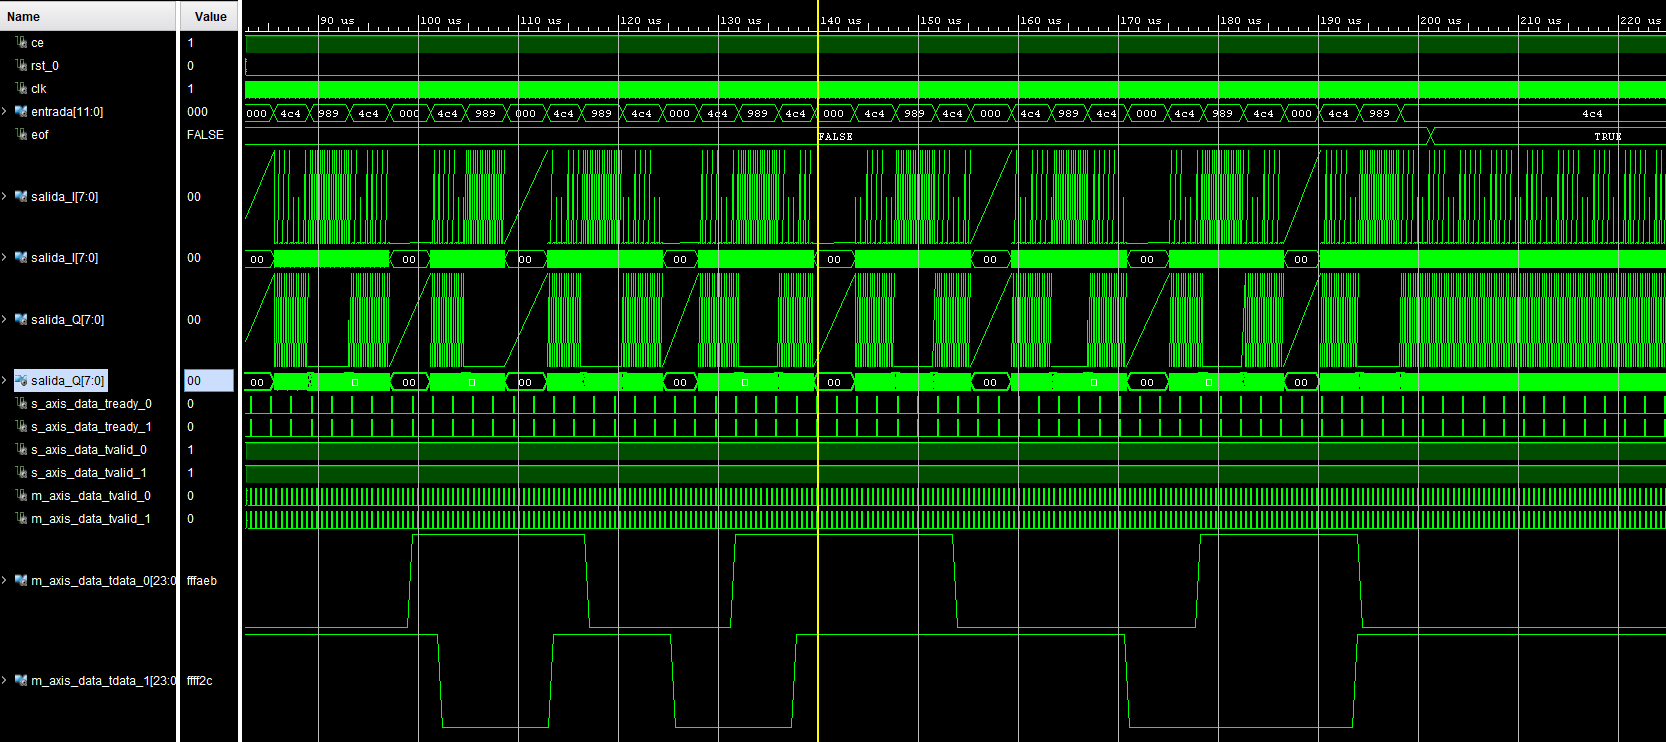
\includegraphics[width=1\textwidth]{img/simu/rrc2.PNG}
	\caption{Simulación de los bloques de mapeado 16-QAM + ZP y filtrado RRC (II)}
	\label{fig:rrc2}
\end{figure}

\vspace{3mm}